
\definecolor{Mred}{HTML}{e71d36}
\definecolor{Mblue}{HTML}{457b9d}
\definecolor{MBlack}{HTML}{011627}
\definecolor{MWhite}{HTML}{fdfffc}
\definecolor{MYellow}{HTML}{ff9f1c}
\definecolor{MGreen}{HTML}{189655}
\tikzstyle{terminator} = [rectangle, draw, text centered, rounded corners, minimum height=2em]
\tikzstyle{connector} = [draw, -latex']



\section{Partie graphique}

La partie graphique de Saint-Nec Engine a pour but d'implémenter différentes fonctionnalités par la création d'exemples concrets. Ainsi, nous avons fait de la génération de terrain, d'herbe et d'eau dans le but de découvrir différentes méthodes de programmation et d'optimisation que nous avons par la suite intégrées directement dans la bibliothèque.

\subsection{Introduction à la programmation graphique}

Dans un logiciel en 3D ou même en 2D, tout est représenté sous la forme d'un assemblage de primitives (des triangles ou des carrés). L'association de plusieurs triangles permet de représenter n'importe quel objet, du plus simple au plus complexe, et de manière plus ou moins détaillée. Chaque primitive est composée de sommets (3 dans le cas d'un triangle) reliées entre elles. Par dessus cette primitive, nous pouvons alors dessiner des couleurs ou des textures (par exemple des images).

Pour afficher un objet à l'écran, il faut dans un premier temps définir l'ensemble des primitives que l'on souhaite afficher et leurs donner des positions dans l'espace. Ensuite, nous envoyons toutes ces données à la carte graphique (\textit{Graphics Processing Unit} ou GPU) et quand nous voulons les afficher, on exécute un \og Draw call \fg ou appel à dessiner qui va dire à notre GPU qu'il faut afficher cet objet.

\begin{figure}[H]
	\begin{minipage}[t!]{0.50\textwidth} % Zone de texte à gauche (60% de la largeur de la page)
		Une fois que l'on demande à dessiner notre objet, il passe dans la pipeline graphique, ce qui permet de transformer toutes nos données en un élément visible à l'écran. Ces étapes nommées shaders sont des petits programmes s'exécutant sur notre carte graphique. Les deux principaux shaders modifiables que l'on peut voir dans la \autoref{fig:pipelineGr} s'exécutent dans un ordre bien précis:
		\begin{itemize}
			\item Le vertex shader a pour but de transformer toutes les coordonnées de nos primitives envoyées plus tôt dans le repère de l'écran. Cela s'effectue grâce à la multiplication de matrices élémentaires représentant notre caméra et notre \og monde\fg.
			\item Le fragment shader lui s'exécute pour chaque pixel visible à l'écran d'un objet. Son but est de déterminer la couleur de ce pixel (c'est ici qu'on peut afficher notre image ou notre couleur).
		\end{itemize}
	\end{minipage}
	\hfill % Espace horizontal flexible pour séparer l'image et le texte
	\begin{minipage}[t!]{0.45\textwidth} % Zone d'image à droite (35% de la largeur de la page)
		\begin{figure}[H]	
			\centering		
			\begin{tikzpicture}
				\node [terminator, fill=MGreen!20] at (0,0) (vertex) {\textbf{Vertex}};
				\node [terminator, fill=MGreen!20] at (0,-4) (fragment) {\textbf{Fragment}};
				
				
				\path [connector] (vertex) -- (fragment);

			\end{tikzpicture}
			\caption{Pipeline graphique simplifiée}
			\label{fig:pipelineGr}
		\end{figure}
	\end{minipage}
\end{figure}


\subsection{Génération de terrain}

Dans chaque jeu vidéo en 3D, le joueur évolue dans un environnement. Celui-ci peut être vaste et est visible par le joueur à tout moment pour ne pas rompre l'immersion. Dans la plupart des jeux en monde ouvert comme dans la \autoref{fig:zeldabotw}, on est capable de distinguer les montagnes même si elles sont très loin. Le but de cette partie a alors été de comprendre comment les jeux vidéo font pour avoir un terrain si vaste et si détaillé tout en étant fluide.

\begin{figure}[!h]			
	\centering{\includegraphics[width=130mm]{Image/Graphique/zelda_botw.jpg}}
	\caption{Capture d'écran de \og The Legend of Zelda: Breath of the Wild\fg}
	 \label{fig:zeldabotw}
\end{figure}

\subsubsection{Création à partir de carte de hauteur}

La première étape a été de créer notre terrain. Nous avons ainsi créé un plan horizontal composé de milliers de sommets. Ensuite, nous déplaçons chaque sommets selon l'axe vertical afin de donner de la hauteur. Pour ce faire, nous avons utilisé une carte de hauteur (\autoref{fig:noise}), le gradient de couleur représente la hauteur et plus la couleur de notre carte est blanche, plus le point associé est haut. 

\begin{figure}[H]			
	\centering{\includegraphics[width=50mm]{Image/Graphique/Terrain/noise.jpg}}
	\caption{Exemple de carte de hauteur}
	\label{fig:noise}
\end{figure}

Nous appliquons donc cette image à notre plan (\autoref{fig:terrainBasique}) et nous déplaçons nos sommets pour donner le relief à notre terrain (\autoref{fig:terrainHauteur}). Pour faire cela, nous avons créé un Vertex shader qui pour chaque sommet du plan, récupère la valeur en niveau de gris associée à ce point dans la carte de hauteur. Ensuite, nous avons juste à déplacer le sommet selon l'axe vertical en fonction de la valeur de ce niveau de gris.
\pagebreak
\begin{figure}[H]			
	\centering{
		\includegraphics[width=130mm]{Image/Graphique/Terrain/terrain.png}
		}
	
	\caption{Plan avec la carte de hauteur}
	\label{fig:terrainBasique}
\end{figure}

\begin{figure}[H]			
	\centering{

		\includegraphics[width=130mm]{Image/Graphique/Terrain/terrainHauteur.png}
	}
	
	\caption{Plan avec la carte de hauteur et déplacement des sommets}
	\label{fig:terrainHauteur}
\end{figure}
Cette méthode est très simple à implémenter, mais comporte plusieurs désavantages. L'information en niveau de gris est stockée sous la forme d'un entier sur 8 bits ce qui représente 256 valeurs possibles. De ce fait, la précision que l'on veut donner à notre terrain est assez limitée. Cependant, cela rend son stockage assez efficace vu que nous ne stockons que 8 bits par sommets. De plus, cette technique ne permet pas d'avoir plusieurs points pour une même coordonnée horizontal, nous ne pouvons par exemple pas dessiner une grotte qui demande d'avoir un plafond et un sol.

\pagebreak
\subsubsection{Ajout de texture}

Maintenant que nous avons de la hauteur, nous pouvons ajouter de la couleur. Pour modifier la couleur d'un sommet, nous passons par le fragment shader. Nous avons décidé de peindre notre terrain selon la hauteur de chaque sommets et utilisons deux textures (\autoref{fig:terrainTextures}) représentant de l'herbe et de la terre. Ainsi, plus le sommet est haut, plus il aura la couleur de l'herbe et plus il est bas, plus ce sera de la terre. Le résultat de ce mélange des deux texture est visible sur la \autoref{fig:terrainCouleur}.
\begin{figure}[H]			
	\centering{
		\includegraphics[width=50mm]{Image/Graphique/Terrain/grass.jpg}
		\hskip 5pt
		\includegraphics[width=50mm]{Image/Graphique/Terrain/rock.jpg}
		}
	
	\caption{Textures utilisées pour le terrain}
	\label{fig:terrainTextures}
\end{figure}

L'ajout de couleur à notre terrain se fait dans un fragment shader. Ici, pour chaque pixel du terrain, nous récupérons la valeur de la texture associée pour l'herbe et la terre et ensuite nous faisons une interpolation linéaire entre les deux couleurs en fonction de la valeur de hauteur de notre point.

\begin{figure}[H]			
	\centering{
		
		\includegraphics[width=130mm]{Image/Graphique/Terrain/terrainCouleur.png}
	}	
	\caption{Terrain texturé}
	\label{fig:terrainCouleur}
\end{figure}

Cette méthode pour peindre le terrain est peu coûteuse en termes de temps de calcul mais est peu personnalisable. En effet, dans la plupart des cas, nous souhaitons avoir un plus grand contrôle sur la texture utilisée et donc dessiner à la main sur le terrain pour avoir plus de détail et de diversité.

\subsubsection{Optimisation par niveau de détail}

Si nous souhaitons avoir plus de détail sur notre terrain, nous augmentons la densité de celui-ci en rajoutant plus de sommets \footnote{\url{https://www.youtube.com/watch?v=4_0hg54vT2w}}. Cependant, cela augmente les temps de calcul et réduit ainsi les performances. Dans la \autoref{fig:terrainCouleur}, nous ne pouvons pas distinguer tous les détails du terrain éloignés de la caméra mais pourtant ceux-ci sont calculés à chaque fois. La carte graphique n'est donc pas utilisée de manière optimale. C'est là qu'intervient le niveau de détail (\textit{Level of detail} ou LOD). Son but est de maximiser le détail des objets proches de la caméra (et donc visibles) mais aussi de le réduire pour les objets éloignés. 








\begin{figure}[H]
	\begin{minipage}[t!]{0.50\textwidth} % Zone de texte à gauche (60% de la largeur de la page)
		Pour notre terrain, nous allons utiliser la tessellation. Son but est, à partir d'un carré, de le subdiviser en plein de triangles. La tessellation est une étape de la pipeline graphique située entre le vertex et le fragment shader comme montré dans la \autoref{fig:pipelineTess}. La tessellation est composée de 3 étapes dont 2 que l'on peut contrôler grâce à des shaders : le contrôle et l'évaluation.
		
		L'étape de contrôle permet de définir le nombre de subdivisions pour un carré. La génération de primitive sert à créer de nouveaux sommets au sein de notre carré. Enfin, durant l'évaluation, nous plaçons ces sommets dans notre carré. 
	\end{minipage}
	\hfill % Espace horizontal flexible pour séparer l'image et le texte
	\begin{minipage}[t!]{0.45\textwidth} % Zone d'image à droite (35% de la largeur de la page)
		\begin{figure}[H]			
			\begin{tikzpicture}
				\node [terminator, fill=MGreen!20] at (0,0) (vertex) {\textbf{Vertex}};
				\node [terminator, fill=blue!20] at (0,-2) (control) {\textbf{Tessellation Control}};
				\node [terminator, fill=blue!20] at (0,-4) (primitive) {\textbf{Tessellation Primitive Generator}};		
				\node [terminator, fill=blue!20] at (0,-6) (eval) {\textbf{Tessellation Evaluation}};
				\node [terminator, fill=MGreen!20] at (0,-8) (fragment) {\textbf{Fragment}};
				
				
				\path [connector] (vertex) -- (control);
				\path [connector] (control) -- (primitive);
				\path [connector] (primitive) -- (eval);
				\path [connector] (eval) -- (fragment);
			\end{tikzpicture}
			\caption{Pipeline graphique avec la tessellation}
			\label{fig:pipelineTess}
		\end{figure}
	\end{minipage}
\end{figure}



On peut subdiviser chaque carré en fonction de deux paramètres : le nombre de subdivisions internes et externes notés $i$ et $e$ (dans chaque cas expérimenté $i$ = $e$). Dans la \autoref{fig:terrainTess}, on peut observer le résultat de la tessellation d'un carré pour plusieurs valeurs. Dans notre cas, plus $i$ et $e$ sont grands, plus le terrain sera détaillé.
\begin{figure}[H]			
	\centering{
		\begin{minipage}[t!]{0.32\textwidth}
			\includegraphics[width=50mm]{Image/Graphique/Terrain/tessNiveau0.png}
			\centering
			$i$ = $e$ = 1 
		\end{minipage}
		\begin{minipage}[t!]{0.32\textwidth}
			\includegraphics[width=50mm]{Image/Graphique/Terrain/tessNiveau4.png}
			\centering
			$i$ = $e$ = 4
		\end{minipage}
		\begin{minipage}[t!]{0.32\textwidth}
			\includegraphics[width=50mm]{Image/Graphique/Terrain/tessNiveau11.png}
			\centering
			$i$ = $e$ = 11
		\end{minipage}
	}	
	\caption{Terrain avec des textures}
	\label{fig:terrainTess}
\end{figure}

Maintenant, pour créer ce niveau de détail, nous calculons la distance entre la caméra et chaque carré. Plus cette distance est grande, moins le carré sera subdivisé. Cela nous permet d'avoir un niveau de détail dynamique et de limiter la perte d'information à la caméra. On peut voir le résultat dans la \autoref{fig:exTess} où le centre de l'image a été plus divisé que l'extérieur car il est plus proche de la caméra.

\begin{figure}[H]			
	\centering{
		
		\includegraphics[width=130mm]{Image/Graphique/Terrain/exTess.png}
	}	
	\caption{Exemple de tessellation en fonction de la distance de la caméra}
	\label{fig:exTess}
\end{figure}

Étant donné que la subdivision se fait en temps réel, si les paramètres ne sont pas bien choisis, nous pouvons avoir un effet de \og popping\fg où l'on voit des sommets apparaitre devant la caméra et cassant l'immersion\footnote{\url{https://www.youtube.com/watch?v=FHJPCFyHV9c}}. Il faut alors choisir la bonne distance à partir de laquelle nous commençons à subdiviser notre terrain pour ne pas détériorer la qualité graphique tout en améliorant les performances.

\subsubsection{Effet de la tessellation sur les performances}

Pour mesurer l'effet sur les performances du notre terrain avec et sans tessellation, il faut trouver les bons paramètres de tessellation afin que la différence visuelle entre les deux versions soit la plus minime possible. Nous pouvons alors modifier 2 paramètres décrits dans le \autoref{tab:tabVarTess}. 



\begin{table}[H]
	\centering
	\begin{tabular}{|c|l|}
		\hline
		\textbf{Nom de la variable} & \textbf{Description}  \\
		\hline
		$S_{max}$ & Nombre maximum de subdivisions\\
		$D$ & Distance maximale à laquelle on subdivise nos carrés\\
		\hline
	\end{tabular}
	\caption{Tableau des variables pour la tessellation}
	\label{tab:tabVarTess}
\end{table}

Pour nos mesures, nous avons positionné la caméra au centre d'un terrain de 300 par 300 avec pour la tessellation nos variables $S_{max}$=12 et $D$=150. Nous comparons ces paramètres avec un terrain de 300 par 300 mais avec une densité initiale 36 fois supérieure. Nous avons choisi ces paramètre au jugé pour représenter au mieux la vision d'un joueur. Ainsi, à travers des tests, nous avons définit ces différents paramètres comme équivalent.

Pour déterminer l'effet de la tessallation, nous avons mesuré les performances du programme en fonction des divers paramètres décrits précédemment. Nous avons mesuré la moyenne d'images par secondes (IPS) de notre programme sur 30 secondes avec la caméra fixe située au milieu du terrain. Nous mesurons les IPS car c'est la méthode la plus utilisée pour vérifier qu'un jeu est suffisamment fluide.

La configuration de test est un Lenovo Legion Y520-15IKBM avec un processeur Intel i5 7300hq, 16go de RAM en DDR4 2400MHz et une Nvidia GTX 1060 max-q 6go. Pour donner un ordre d'idée, on considère un jeu fluide quand il tourne à au moins 60 IPS (plus il y en a, mieux c'est).


Nous obtenons alors une moyenne de 585 images par secondes dans le cas du terrain non optimisé contre 1082 de moyenne pour le terrain avec la tessellation. Nous obtenons alors une amélioration de 84~\% de nos performances grâce à la tessellation. Plus le terrain va être grand, plus cette simple optimisation va avoir un effet positif sur les performances vu que l'on augmente la définition du terrain en temps réel autour du joueur au lieu de toujours tout afficher.


\pagebreak
\subsection{Génération d'herbe}

Dans les jeux vidéo modernes et se voulant réaliste, l'herbe est un élément essentiel pour améliorer l'immersion et le détail apporté à l'environnement. Implémenter la génération d'herbe permet aussi de voir plusieurs techniques d'optimisation que nous décrirons plus tard. Nous nous sommes basés sur les travaux des équipes de Sucker Punch Production pour le rendu de l'herbe grâce à leurs Game Developer Conference Talk \og Advanced Graphics Summit: Procedural Grass in 'Ghost of Tsushima'\fg \citep{herbe} de 2021.

\subsubsection{Création d'un brin d'herbe}

Premièrement, un brin d'herbe est un objet créé à partir d'une géométrie. Cet objet étant affiché des centaines de milliers de fois au même moment, sa géométrie ne peut pas être trop détaillée car sinon le jeu ne serait pas fluide. De ce fait, nous avons décidé de générer un brin d'herbe à partir de 7 triangles (\autoref{fig:brin_herbe}). Ce nombre a été choisi arbitrairement pour avoir suffisamment de détails sans être trop complexe.
\begin{figure}[!h]
	\begin{center}
		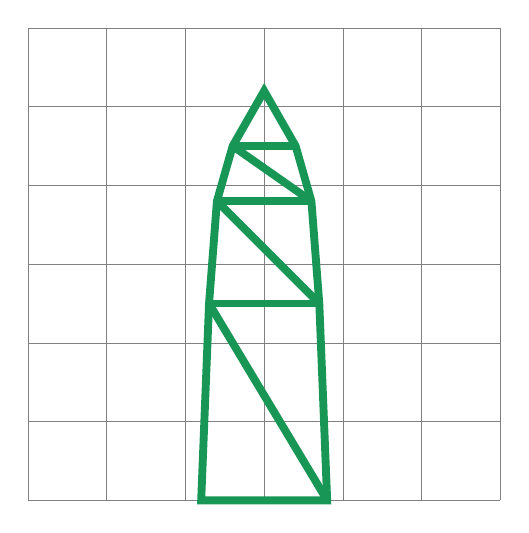
\begin{tikzpicture}
			\draw[step=1cm,gray,very thin] (0,0) grid (6,6);
			\draw[MGreen, line width=1mm] (2.2,0) -- (2.3,2.5) -- (2.4,3.8) -- (2.6,4.5) -- (3,5.2) -- (3.4,4.5) -- (3.6,3.8) -- (3.7,2.5) -- (3.8,0) -- cycle;
			
			\draw[MGreen, line width=1mm] (2.3,2.5) -- (3.8,0);
			\draw[MGreen, line width=1mm] (2.3,2.5) -- (3.7,2.5);
			
			\draw[MGreen, line width=1mm] (2.4,3.8) -- (3.7,2.5);
			\draw[MGreen, line width=1mm] (2.4,3.8) -- (3.6,3.8);
			
			\draw[MGreen, line width=1mm] (2.6,4.5) -- (3.6,3.8);
			\draw[MGreen, line width=1mm] (2.6,4.5) -- (3.4,4.5);
			
		\end{tikzpicture}
	\end{center}
	\caption{Géométrie d'un brin d'herbe}
	\label{fig:brin_herbe}
\end{figure}

Chaque brin d'herbe possède donc 9 sommets et tout ces sommets possèdent un vecteur normal (vecteur perpendiculaire à la face de notre objet) qui nous sera utile plus tard pour l'éclairage.

\noindent Une fois la géométrie déterminée, nous pouvons commencer à ajouter de la couleur et du mouvement pour rendre cette prairie avec du vent réaliste. Pour cela nous avons créé une scène avec 100 brins d'herbe pour illustrer ces changements. 
Dans un premier temps, nous disposons ces 100 brins de manière pseudo-aléatoire à la création de la scène. Ainsi, chaque brin possède une position initiale de manière ce qu'ils soient tous équidistants. On ajoute aussi un léger décalage afin de donner cet aspect aléatoire plus naturel. Ensuite, nous donnons deux couleurs à notre brin d'herbe, une pour le bas et une pour le haut et nous interpolons entre ces deux en fonction de la hauteur (\autoref{fig:herbe1}).

\begin{figure}[H]			
	\centering{\includegraphics[width=100mm]{Image/Graphique/Herbe/dep.png}}
	\caption{100 brins d'herbe}
	\label{fig:herbe1}
\end{figure}

Ensuite, nous ajoutons une rotation autours de l'axe vertical (\autoref{fig:herbe2}). Cet angle de rotation est déterminé par une fonction de hachage qui prend en paramètre le numéro d'instance du brin d'herbe et retourne une valeur pseudo-aléatoire.
Pour générer une valeur aléatoire sur notre carte graphique, nous utilisons une fonction de hachage. C'est une fonction qui prend en paramètre un nombre et le transforme de manière à ce qu'il ne ressemble pas au nombre de départ et semble aléatoire. Nous transformons ce nombre en le multipliant par des grands nombres et en faisant des opérations bits à bits comme des \og ou exclusif\fg \ ou des décalages de bits (algorithme \autoref{alg:hash}). Même si cette fonction est basique et que l'aléatoire en sortant est prévisible, cela reste amplement suffisant pour servir de rotation à nos brins d'herbe. De plus, son temps de calcul est très faible. 

\begin{algorithm}[H]
	\caption{Exemple de fonction de hachage simple}
	\label{alg:hash}
	\begin{algorithmic}
		\Require{$x$: nombre à transformer}	
		\State $x \gets x\oplus (x >>16)$
		\State $x \gets x\times 0x7feb352dU$
		\State $x \gets x\oplus (x >>15)$
		\State $x \gets x\times 0x846ca68bU$
		\State $x \gets x\oplus (x >>16)$
		
		\State \textbf{return} x
	\end{algorithmic}
\end{algorithm}



\begin{figure}[H]			
	\centering{\includegraphics[width=100mm]{Image/Graphique/Herbe/dep+rot.png}}
	\caption{100 brins d'herbe avec rotation}
	\label{fig:herbe2}
\end{figure}

Dans la vraie vie, les brins d'herbes ne sont pas totalement droits. Pour simuler ce comportement, nous appliquons une rotation sur l'axe parallèle à notre brin d'herbe avant celle autour de l'axe vertical (visible sur la \autoref{fig:herbe3}). L'ordre de ces opérations est important car nous travaillons avec des matrices et la multiplication matricielle n'est pas une opération commutative. Dans notre cas, nous voulons d'abord courber notre brin d'herbe avant de le tourner.  Cette rotation est aussi déterminée avec une fonction de hachage.

\begin{figure}[H]			
	\centering{\includegraphics[width=100mm]{Image/Graphique/Herbe/dep+rot+curv.png}}
	\caption{100 brins d'herbe avec rotation et courbure de l'herbe}
	\label{fig:herbe3}
\end{figure}

Notre brin d'herbe est défini sur 2 dimensions donc si on positionne la caméra pour qu'elle soit parallèle à notre brin, celui-ci ne sera pas visible. Avoir un brin d'herbe non visible utilise de la puissance de calcul pour rien. Alors, quand la caméra s'approche de cette position critique, nous ajoutons une petite rotation sur l'axe vertical afin de recentrer ce brin pour qu'il soit visible le plus longtemps possible à la caméra. Si on compare la \autoref{fig:herbe3} avec la \autoref{fig:herbe4} qui met en place cet effet, on peut voir que cette rotation rend la scène plus dense. Pour obtenir la même densité sans cet effet, il aurait fallu ajouter plus de brins d'herbe à la scène, ayant un coût supplémentaire sur les performances.  

\begin{figure}[H]			
	\centering{\includegraphics[width=100mm]{Image/Graphique/Herbe/dep+rot+curv+adj.png}}
	\caption{100 brins d'herbe avec rotation, courbure de l'herbe et ajustement par rapport à la caméra}
	\label{fig:herbe4}
\end{figure}


Dernièrement, pour rendre la scène plus réaliste, nous avons ajouté un effet de lumière directionnelle. C'est une lumière qui émet dans un seul sens. Ce type de lumière est souvent utilisé pour simuler le soleil dans un jeu. Ainsi, plus le brin d'herbe est face à la lumière, plus celui-ci va être éclairé et inversement (\autoref{fig:herbe5})

\begin{figure}[H]			
	\centering{\includegraphics[width=100mm]{Image/Graphique/Herbe/dep+rot+curv+adj+col.png}}
	\caption{100 brins d'herbe avec gestion de la lumière}
	\label{fig:herbe5}
\end{figure}



\noindent D'un point de vu algorithmique, ce calcul est divisé en 3 étapes:
\begin{itemize}
	\item Retrouver quelle face du brin d'herbe est visible à la caméra
	\item Recalculer le vecteur normal par rapport à la face affichée
	\item Calculer l'impact de la lumière sur le brin d'herbe.
\end{itemize}
\noindent Dans l'algorithme \autoref{alg:lumiere}, $sign$ est une fonction retournant -1 si la valeur est négative et 1 sinon. Et la fonction $max$ retourne le plus grand des deux nombres passés en paramètres. Ici, en passant en paramètre de cette fonction notre valeur de lumière et 0, on enlève les valeurs correspondant à un éclairage négatif (et qui n'ont donc pas de sens dans notre cas).
\begin{algorithm}[H]
	\caption{Calcul de la valeur de lumière diffuse pour un pixel}
	\label{alg:lumiere}
	\begin{algorithmic}
		\Require{$cameraFront$ : Vecteur de direction de la caméra, $normal$ : vecteur normal du brin d'herbe}	
		\State $faceRendered \gets cameraFront \cdot normal$
		\State $visibleNormal \gets normal \times sign(faceRendered)$ 
		\State $diffuse \gets max(visibleNormal \cdot lightDirection, 0.0)$
		
		\State $\textbf{return} \ diffuse$
	\end{algorithmic}
\end{algorithm}

Pour simuler l'effet du vent sur notre scène, le but est de bouger chaque brin d'herbe dans un sens avec une intensité définie. Le sens du vent est un vecteur défini sur les 2 axes horizontaux. Pour donner l'effet, il faut un moyen de faire varier l'intensité du vent en fonction du temps. La méthode la plus simple est alors d'utiliser une fonction sinus ou cosinus car ces fonctions sont périodiques avec des valeurs comprises entre -1 et 1. En calculant le sinus avec la position du brin d'herbe et le temps, nous sommes capables d'obtenir un effet de vent sur notre champ d'herbe. Cependant, ce mouvement simple et uniforme et ne semble pas très naturel\footnote{\url{https://www.youtube.com/watch?v=wZaexk1z9ng}}. Ceci est dû à la nature périodique de la fonction sinus qui se répète à l'identique dans le temps.

Une autre approche pour simuler cet effet de manière plus réaliste est d'utiliser du bruit. Nous utilisons alors du bruit de Perlin pour donner cet effet plus naturel au mouvement du vent\footnote{\url{https://www.youtube.com/watch?v=Ft2P-KOoZWY}}. Le bruit de Perlin est un bruit de gradient décrit pour la première fois par Kenneth Perlin dans \og An image synthesizer\fg\citep{perlin} permettant la création de valeur pseudo-aléatoires comme dans la \autoref{fig:noise} pour représenter notre terrain. En fonction de la valeur du bruit, nous déplaçons les sommets des brins d'herbe dans la direction du vent. Grâce à l'ajout de bruit, les mouvements paraissent plus aléatoires et donc plus naturels.

\subsubsection{Optimisation par \og instancing\fg}

Actuellement, à chaque nouvelle image que le programme calcul, nous demandons à la carte graphique de dessiner les brins d'herbe un par un. Cependant, pour que la scène semble réaliste, nous voulons dessiner des centaines de milliers de brins en même temps, ce qui va réduire considérablement les performances de notre programme. Quand on demande à notre carte graphique de dessiner un objet dans la scène (les \og Draw Calls\fg), le processeur va envoyer toutes les données nécessaires à leur affichage. Dans notre cas, la plupart des données sont identiques entre chaque brin d'herbe donc on perd du temps de calcul à envoyer des centaines de milliers de fois les mêmes données.
La première solution va être d'utiliser de l'\textit{instancing}. Étant donné que chaque brin d'herbe utilise la même géométrie, l'\textit{instancing} permet de demander à la carte graphique de dessiner tous nos brins d'herbe en une seule fois. Ainsi, on évite d'envoyer plusieurs fois les mêmes informations et on augmente de manière significative les performances de notre application. Au niveau du code, on remplace tous nos appels à dessiner par un seul.



\subsubsection{Optimisation par niveau de détail}

Comme pour la génération de terrain, les brins d'herbe éloignés de la caméra ne représentent que quelques pixels sur l'écran et donc avoir un brin très détaillé n'est pas utile. Cette fois-ci, au lieu de rajouter du détail quand la caméra est proche de l'objet, nous allons au contraire réduire sa qualité en fonction de son éloignement. Nous définissons alors différentes géométries plus ou moins détaillées de notre brin d'herbe comme on peut le voir dans la \autoref{fig:brin_herbe_lod}. Ici nous avons deux maillages, le plus détaillé étant composé de 7 triangles et le deuxième de seulement 1. Ensuite, pour décider lequel des deux maillages afficher, on calcule la distance entre la caméra et le brin et on définit un seuil arbitraire à partir duquel on change le maillage à afficher.



\begin{figure}[H]
	\begin{center}
		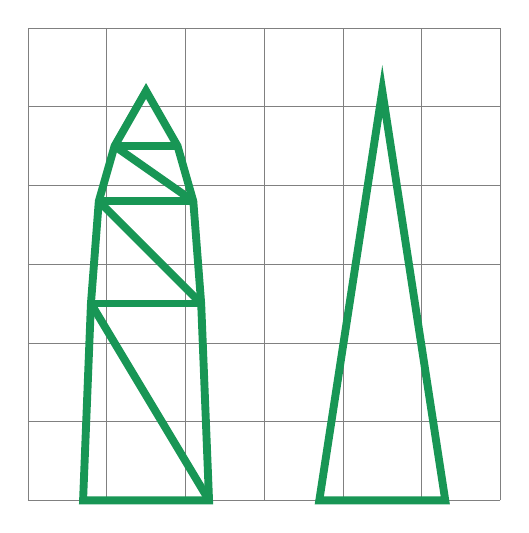
\begin{tikzpicture}
			\draw[step=1cm,gray,very thin] (0,0) grid (6,6);
			\draw[MGreen, line width=1mm] (0.7,0) -- (0.8,2.5) -- (0.9,3.8) -- (1.1,4.5) -- (1.5,5.2) -- (1.9,4.5) -- (2.1,3.8) -- (2.2,2.5) -- (2.3,0) -- cycle;
			\draw[MGreen, line width=1mm] (0.8,2.5) -- (2.3,0);
			\draw[MGreen, line width=1mm] (0.8,2.5) -- (2.2,2.5);
			\draw[MGreen, line width=1mm] (0.9,3.8) -- (2.2,2.5);
			\draw[MGreen, line width=1mm] (0.9,3.8) -- (2.1,3.8);
			\draw[MGreen, line width=1mm] (1.1,4.5) -- (2.1,3.8);
			\draw[MGreen, line width=1mm] (1.1,4.5) -- (1.9,4.5);
			
			\draw[MGreen, line width=1mm] (3.7,0) --(4.5,5.2) -- (5.3,0) -- cycle;
		\end{tikzpicture}
	\end{center}
	\caption{Niveau de détail des brin d'herbes}
	\label{fig:brin_herbe_lod}
\end{figure}

\subsubsection{Optimisation par \og view frustum culing\fg}

La dernière optimisation mise en place pour la génération d'herbe est le \textit{view frustum culling} ou élimination des objets hors du cône de vue. C'est un algorithme qui a pour but de ne pas dessiner les objets non visibles par la caméra. Comme expliqué précédemment, demander à la carte graphique de dessiner un objet est coûteux en termes de performance et faire cet appel alors qu'il n'est pas visible est une perte considérable de ressources. 
Dans un jeu, la caméra est définie par un cône de vue à 6 faces, les objets en dehors de ce cône ne sont donc pas visibles à l'écran. Dans la \autoref{fig:frustum culing} représentant une vue en deux dimensions de notre monde, les objets verts situés dans le cône de vision en bleu sont visibles donc on souhaite les dessiner.



\begin{figure}[H]
	\begin{center}
		\begin{tikzpicture}
			\draw[step=1cm,gray,very thin] (0,0) grid (6,6);
			\fill[fill=Mblue, opacity=0.5](1,5) -- (2.2,2) -- (3.8,2) -- (5,5) -- cycle ;
			
			
			\fill[fill=Mred, shift={(3.2,5.1)}, rotate around z=30, scale=0.6] (0,0) -- (1,0.0) -- (1,1) -- (0,1)  ;
			\fill[fill=MGreen, shift={(1.5,2.7)}, rotate around z=350, scale=0.9] (0,0) -- (1,0.0) -- (1,1) -- (0,1)  ;
			\fill[fill=Mred, shift={(4.2,1)}, rotate around z=330, scale=1.2] (0,0) -- (1,0.0) -- (1,1) -- (0,1)  ;
			\fill[fill=MGreen, shift={(3.4,4)}, rotate around z=00, scale=0.7] (0,0) -- (1,0.0) -- (1,1) -- (0,1)  ;
			\fill[fill=Mred, shift={(1.2,0.9)}, rotate around z=00, scale=0.5] (0,0) -- (1,0.0) -- (1,1) -- (0,1)  ;
			
			\node[inner sep=0pt, rotate=90]  at (3,1)
			{\includegraphics[width=.07\textwidth]{Image/Icons/camera.png}};	
		\end{tikzpicture}
	\end{center}
	\caption{Exemple de \og View Frustum Culing\fg}
	\label{fig:frustum culing}
\end{figure}

Pour savoir si un objet est dans le cône de vision de la caméra nous allons utiliser la méthode de Gribb/Hartmann\citep{gribbHartman} permettant de récupérer les 6 plans représentant le cône à partir de la matrice de projection multipliée par la matrice de vue. Dans l'algorithme~\ \autoref{alg:gribbHartmann}, on peut extraire les plans de la caméra de manière très efficace en additionnant ou en soustrayant les lignes de la matrice de vue projection.



\begin{algorithm}[H]
	\caption{Extraction des plans du cône de vision par la méthode Gribb/Hartmann}
	\label{alg:gribbHartmann}
	\begin{algorithmic}
		
		\State $matriceVueProjection \gets vue \times projection$
		\newline
		\State $ligne1 \gets matriceVueProjection[0]$
		\State $ligne2 \gets matriceVueProjection[1]$
		\State $ligne3 \gets matriceVueProjection[2]$
		\State $ligne4 \gets matriceVueProjection[3]$
		\newline
		\State $planGauche \gets ligne1 + ligne4$
		\State $planDroit \gets ligne1 - ligne4$
		\State $planBas \gets ligne2 + ligne4$
		\State $planHaut \gets ligne2 - ligne4$
		\State $planProche \gets ligne3 + ligne4$
		\State $planLoin \gets ligne3 - ligne4$
		
	\end{algorithmic}
\end{algorithm}

Ensuite, nous dessinons notre objet si au moins un de ses sommets est dans le cône de la caméra. Pour que le point soit dans le cône de vision, il doit respecter ces six conditions :
\[planGauche \cdot point \geqslant 0\]
\[planDroit \cdot point \leqslant 0\]
\[planBas \cdot point \geqslant 0\]
\[planHaut \cdot point \leqslant 0\]
\[planProche \cdot point \geqslant 0\]
\[planLoin \cdot point \leqslant 0\]

Cette implémentation du \textit{view frustum culling} est performante car elle ne demande que très peu de calculs, mais elle a un défaut. Comme on peut le voir dans la \autoref{fig:frustum culing_effet_bord}, le cube en vert noté \og 1\fg \ va être dessiné car un de ses sommets est à l'intérieur du cône de vision. Mais le cube en rouge noté \og 2\fg, bien que lui aussi dans le cône de vision, ne sera pas dessiné car aucun de ses sommets est compris dans ce même cône. L'utilisateur va alors voir des objets apparaitre et disparaitre alors qu'ils sont encore dans le champ de vision de la caméra. Ce problème peut être résolu en implémentant une détection de collision plus robuste comme celle utilisée pour la partie physique de notre moteur.

\begin{figure}[H]
	\begin{center}
		\begin{tikzpicture}
			\draw[step=1cm,gray,very thin] (0,0) grid (6,6);

			
			

			\fill[fill=MGreen, shift={(1.0,2.7)}, rotate around z=350, scale=0.9] (0,0) -- (1,0.0) -- (1,1) -- (0,1)  ;
			\fill[fill=Mred, shift={(3.2,1.9)}, rotate around z=300, scale=1.2] (0,0) -- (1,0.0) -- (1,1) -- (0,1)  ;


			\fill[fill=Mblue, opacity=0.5](1,5) -- (2.2,2) -- (3.8,2) -- (5,5) -- cycle ;
			\node[inner sep=0pt, rotate=90]  at (3,1)
			{\includegraphics[width=.07\textwidth]{Image/Icons/camera.png}};
			
			\node[draw] at (1.5,3.05) {1};	
			\node[draw] at (4,1.7) {2};
		\end{tikzpicture}
	\end{center}
	\caption{Effet de bord de l'implémentation du \og View Frustum Culing\fg}
	\label{fig:frustum culing_effet_bord}
\end{figure}

Maintenant, pour implémenter cette technique, il faudrait créer une boite englobante autour de chaque brin d'herbe afin de déterminer si ils sont présents dans le cône de vision. Calculer cela pour des centaines de milliers d'objets est cependant trop coûteux en termes de performance donc nous allons diviser notre scène en tronçons uniformes (chacun contenant un nombre déterminé de brins d'herbe), on appelle chaque tronçon un \textit{chunk}. Ceux-ci vont permettre de réduire considérablement le nombre de calculs nécessaires. Grâce à eux, nous déterminerons si l'on doit afficher ses brins d'herbe et quel niveau de détail leur attribuer.


\pagebreak
\subsubsection{Comparaison des méthodes d'optimisation}

Pour déterminer l'effet des méthodes d'optimisations décrites précédemment, nous avons mesuré les performances du programme en fonction des divers paramètres (\autoref{tabVariablesHerbe}). Nous avons mesuré la moyenne d'images par secondes (IPS) de notre programme sur 30 secondes avec la caméra fixe située au milieu du champ d'herbe. 
Comme pour les tests de perfomances pour la génération de terrain, la configuration de test est un Lenovo Legion Y520-15IKBM avec un processeur Intel i5 7300hq, 16~Go de RAM en DDR4 2400~MHz et une Nvidia GTX 1060 max-q 6~Go. Pour donner un ordre d'idée, on considère un jeu fluide quand il tourne à au moins 60 IPS (plus il y en a, mieux c'est).

\begin{table}[ht]
	\centering
	\begin{tabular}{|c|l|}
		\hline
		\textbf{Nom de la variable} & \textbf{Description}  \\
		\hline
		$S$ & Taille d'un côté de la zone d'herbe\\
		$T$ & Seuil du niveau de détail\\
		$C$ & Taille d'un coté d'un tronçon\\
		$n$ & Nombre de brins d'herbe dans la scène \\
		\hline
	\end{tabular}
	\caption{Tableau des variables pour la génération d'herbe}
	\label{tabVariablesHerbe}
\end{table}

La première mesure a pour but de montrer l'effet de l'\textit{instancing} sur les performances. Dans le \autoref{tab:effetInstancing}, on peut voir que pour un nombre très important d'objets similaires dans une scène, l'instancing est une optimisation simple mais essentielle car elle permet de multiplier par 48 les performances pour 500 000 brins d'herbe. Plus le nombre d'objets à dessiner est grand, plus l'effet de l'\textit{instancing} est important (rapport de 97 pour 1~000~000 d'objets).

\begin{table}[H]
	\centering
	\rowcolors{2}{gray!10}{gray!40}
	\begin{tabular}{|l|l|l|}
		\hline
		
						& $n$=500 000	& $n$=1 000 000 \\ \hline
		Sans instancing &	11,5		&      3,0    	\\
		Avec instancing & 	558,3		&  291,5     \\ \hline
	\end{tabular}
	\caption{Moyenne d'IPS avec et sans instancing, $S$=100}
	\label{tab:effetInstancing}
\end{table}


Ensuite, nous avons fait varier les différents paramètres pour déterminer l'effet de chaque implémentation sur les performances et comment, en combinant ces méthodes, nous pouvons améliorer encore plus le nombre d'IPS du programme. 
Premièrement, on peut observer dans le \autoref{tab:tabPerf2} et le \autoref{tab:tabPerf3} qu'utiliser des tronçons pour diviser notre champ diminue légèrement le nombre d'IPS par rapport à la version avec seulement de l'\textit{instancing}. Cela est dû au fait que l'on doit faire un appel à la carte graphique pour chaque \textit{chunk} au lieu d'un seul pour la version avec instancing.

Quand on ajoute du niveau de détail à notre scène, on augmente nos performances sans réel effet sur la qualité visuelle de notre programme. Logiquement, plus le seuil de distance utilisé est élevé, moins le programme fonctionne rapidement car nous utilisons beaucoup plus le modèle d'herbe détaillé. Cependant, si le seuil utilisé est trop bas, les performances seront meilleures, mais on sera capable de distinguer le modèle d'herbe peu détaillé. Le but est alors, pour les développeurs de jeux vidéo, de trouver le rapport performance/qualité graphique le plus adapté.

L'ajout du \textit{view frustum culling} permet dans chaque cas d'augmenter de manière significative les performances. On remarque aussi que plus le nombre de brins d'herbe est élevé, plus le gain en nombre d'IPS est notable. Dans les mesures, le gain peut aller de 27~\% pour $n$=1 000 000 à 424~\% pour $n$=30 000 000 dans le \autoref{tab:tabPerf4}. On peut remarquer aussi l'effet de la taille des \textit{chunks} en fonction de taille du terrain, c'est alors au développeur du jeu de choisir les bons paramètres en fonction du type de terrain pour son cas d'utilisation.


\begin{table}[H]
	\centering
	\rowcolors{2}{gray!10}{gray!40}
	\begin{tabular}{|l|l|l|l|}
		\hline
		
											& $n$=1 000 000	& $n$=15 000 000 	& $n$=30 000 000 	\\ \hline
		Sans chunk et LOD			 		& 299,4			& 21,1         		& 10,6				\\
		Chunk								& 291,3			& 20,8     			& 10,3				\\
		Chunk + LOD T=50					& 514,5			& 37,4     			& 18,6				\\
		Chunk + LOD T=100					& 331,5			& 23,7				& 11,8				\\
		Chunk + LOD T=50 + Frustum Culling	& 1145,2		& 124,9				& 64,0				\\ \hline
	\end{tabular}
	\caption{Moyenne d'IPS avec instancing, $S$=200 et $C$=10}
	\label{tab:tabPerf2}
\end{table}


\begin{table}[H]
	\centering
	\rowcolors{2}{gray!10}{gray!40}
	\begin{tabular}{|l|l|l|l|}
		\hline
		
											& $n$=1 000 000	& $n$=15 000 000 	& $n$=30 000 000 	\\ \hline
		Sans chunk et LOD					& 299,4			& 21,1         		& 10,6				\\
		Chunk								& 295,3			& 20,8         		& 10,4				\\
		Chunk + LOD T=50					& 514,4			& 37,4         		& 18,7				\\
		Chunk + LOD T=100					& 356,8			& 25,3				& 12,6				\\
		Chunk + LOD T=50 + Frustum Culling	&	1229,5		& 97,0				& 49,7				\\ \hline
	\end{tabular}
	\caption{Moyenne d'IPS avec instancing, $S$=200 et $C$=40}
	\label{tab:tabPerf3}
\end{table}


\begin{table}[H]
	\centering
	\rowcolors{2}{gray!10}{gray!40}
	\begin{tabular}{|l|l|l|l|}
		\hline
		
											& $n$=1 000 000		& $n$=15 000 000 	& $n$=30 000 000 	\\ \hline
		Sans chunk et LOD			 		& 303,3				& 21,5         		& 10,7				\\
		Chunk + LOD T=50					& 564,5				& 43,8         		& 22,1				\\
		Chunk + LOD T=50 + Frustum Culling	& 721,5				& 183,5				& 93,9				\\ \hline
	\end{tabular}
	\caption{Moyenne d'IPS avec instancing, $S$=400 et $C$=10}
	\label{tab:tabPerf4}
\end{table}


\begin{table}[H]
	\centering
	\rowcolors{2}{gray!10}{gray!40}
	\begin{tabular}{|l|l|l|l|}
		\hline
		
											& $n$=1 000 000	& $n$=15 000 000 	& $n$=30 000 000 	\\ \hline
		Sans chunk et LOD					& 303,3			& 21,5         		& 10,7				\\
		Chunk + LOD T=50					& 597,7			& 43,7         		& 21,9				\\
		Chunk + LOD T=50 + Frustum Culling	&	1364,7		& 143,5				& 73,7					\\ \hline
	\end{tabular}
	\caption{Moyenne d'IPS avec instancing, $S$=400 et $C$=40}
	\label{tab:tabPerf5}
\end{table}














\pagebreak
\subsection{Simulation d'un océan}

Pour simuler un océan en programmation graphique, il existe plusieurs méthodes plus ou moins complexes. Nous nous sommes basés sur le livre GPU gems de NVIDIA et du chapitre \og Effective Water Simulation from Physical Models\fg \citep{eau} pour simuler l'effet d'eau et de vagues. Dans un premier temps, nous avons implémenté les méthodes \textit{Sum of Sines}  puis \textit{Gerstner waves} pour le mouvement des vagues et nous avons amélioré le rendu en utilisant le modèle Blinn Phong\cite{blinn} pour éclairer la scène.

\subsubsection{Somme des sinus}
Comme son nom l'indique, cette technique pour simuler le mouvement d'un océan est basée sur la somme de fonctions sinus. Nous utilisons un sinus comme représentant une vague. Chaque vague est composée comme ceci:

\[W(x,z,t) = A \times sin( D \cdot (x, z) \times w + t \times \phi)\]
\newline
Avec comme paramètres:
\begin{itemize}
	\item $A$: amplitude de la vague
	\item $D$: direction de la vague
	\item $w$: longueur d'onde de la vague
	\item $t$: temps (commun à chaque vague)
	\item $\phi$: phase de la vague.
\end{itemize}

Pour obtenir un effet d'océan réaliste, il faut alors additionner plusieurs fonctions sinus en faisant varier les différents paramètres comme on peut le voir dans la \autoref{fig:sumOfSinePlot}.


\begin{figure}[H]
	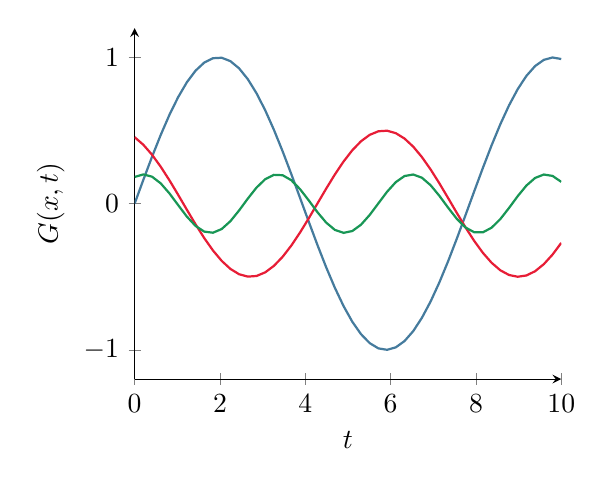
\begin{tikzpicture}
		\begin{axis}[
			axis lines = left,
			xlabel = \(t\),
			ylabel = {\(G(x,t) \)},
			ymin=-1.2, ymax=1.2,
			xmin=0,xmax=10,
			width=7cm,   
			]
			\addplot[samples=50,domain=0:10,domain y=-2:2,color=Mblue,thick]	{sin(deg(x*0.8))};
			\addplot[samples=50,domain=0:10,domain y=-2:2,color=Mred,thick]		{0.5 * sin(deg(x + 2))};
			\addplot[samples=50,domain=0:10,domain y=-2:2,color=MGreen,thick]	{0.2 * sin(deg(x*2+20))};
		\end{axis}
	\end{tikzpicture}
	\hskip 5pt
	\begin{tikzpicture}
		\begin{axis}[
			axis lines = left,
			xlabel = \(t\),
			ylabel = {\(\Sigma  G(x,t)\)},
			ymin=-1.2, ymax=1.2,
			xmin=0,xmax=10,
			width=7cm,   
			]
			\addplot[samples=50,domain=0:10,domain y=-2:2,color=Mblue,thick]	{sin(deg(x*0.8))+0.5 * sin(deg(x + 2))+0.2 * sin(deg(x*2+20))};
		\end{axis}
	\end{tikzpicture}
	\caption{Exemple de somme de sinus en 2D}
	\label{fig:sumOfSinePlot}
\end{figure}

Pour implémenter cet effet, nous avons créé un vertex shader qui va déplacer les points d'un plan verticalement selon la somme des sinus en ce point. On peut voir un résultat de cette implémentation dans la \autoref{fig:sumOfSineImage}.

\begin{figure}[H]			
	\centering{\includegraphics[width=130mm]{Image/Graphique/Eau/SumOfSine.png}}
	\caption{Exemple d'implémentation des sommes de sinus}
	\label{fig:sumOfSineImage}
\end{figure}

Quand la caméra est au bord de l'eau, l'effet est plutôt réussi. Cependant, si on prend de la hauteur dans la scène comme sur la \autoref{fig:sumOfSineImage2}, on peut observer un problème qui détériore considérablement l'effet: la répétition des vagues. En effet, l'une des propriétés de la fonction sinus est sa périodicité donc sa répétition à travers le temps. L'une des solutions serait d'ajouter plus de vague à notre scène mais plus on en ajoute, plus les performances en seront affectées. Il existe plusieurs optimisations possibles pour limiter ce coût comme le niveau de détail mais par manque de temps, nous n'avons pas pu aborder ce sujet pour la simulation d'océan.

\begin{figure}[H]			
	\centering{\includegraphics[width=130mm]{Image/Graphique/Eau/SumOfSineDeHaut.png}}
	\caption{Exemple d'implémentation des sommes de sinus vu d'en haut}
	\label{fig:sumOfSineImage2}
\end{figure}
\pagebreak
\subsubsection{Houle trochoïdale}
L'un des reproches que l'on peut faire à la somme des sinus au niveau graphique est que les vagues semblent un peut trop arrondies. L'une des solutions est d'utiliser des houles trochoïdales ou vagues de Gerstner découvertes en 1802 par Franz Josef Gerstner\citep{gerstner}. De par leur formule mathématique, elles permettent d'avoir une fonction périodique avec des pentes plus abruptes (\autoref{fig:gerstnerImage}) rendant l'effet de fluide plus réaliste. Étant périodiques, elles possèdent le même désavantage que la fonction sinus : la répétition.

\begin{figure}[H]			
	\centering{\includegraphics[width=130mm]{Image/Graphique/Eau/Gerstner.png}}
	\caption{Exemple d'implémentation des vagues de Gerstner}
	\label{fig:gerstnerImage}
\end{figure}

Cet effet de pente plus abrupte est dû au déplacement des sommets sur le plan horizontal en plus du déplacement vertical. Cela a pour effet de rapprocher les sommets horizontalement plus la vague est haute donc augmenter la pente de la vague.

\[G(x,y,t) =\begin{bmatrix}
	x + Q \times A \times D.x \times cos(w \times D \cdot (x,z) + t \times \phi)\\
	A sin(w \times D \cdot (x,z) + t \times \phi)\\
	z + Q \times A \times D.z \times sin(w \times D \cdot (x,z) + t \times \phi)
\end{bmatrix} \]


Avec comme paramètres:
\begin{itemize}
	\item $A$: amplitude de la vague
	\item $D$: direction de la vague
	\item $w$: longueur d'onde de la vague
	\item $t$: temps (commun à chaque vague)
	\item $\phi$: phase de la vague
	\item $Q$: pente de la vague.
\end{itemize}
\pagebreak

Comme on peut le voir dans la \autoref{fig:gerstnerWavePlot}, tout comme pour la somme des sinus, le but de la méthode est de créer plusieurs vagues et de les additionner pour obtenir une simulation d'océan.
\begin{figure}[H]
	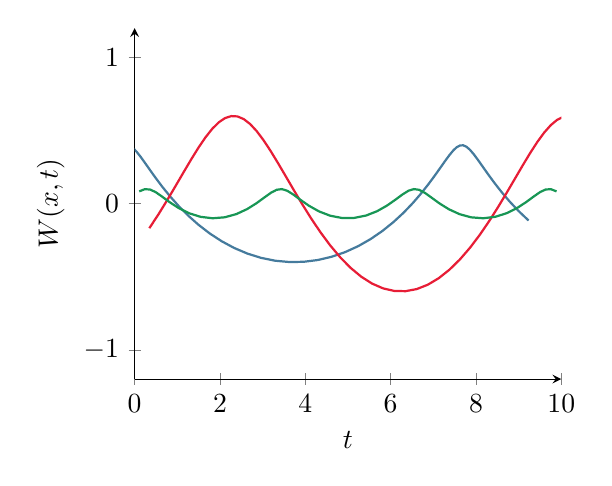
\begin{tikzpicture}
		\begin{axis}[
			axis lines = left,
			xlabel = \(t\),
			ylabel = {\(W(x,t) \)},
			ymin=-1.2, ymax=1.2,
			xmin=0,xmax=10,
			width=7cm,   
			]
			\addplot[samples=50,domain=0:10,domain y=-2:2,color=Mblue,thick]({x+2*0.4 * cos(deg( 8+x*0.8))},{0.4 * sin(deg(8 + x*0.8))});
			\addplot[samples=50,domain=0:10,domain y=-2:2,color=Mred,thick]({x+0.6*0.6 * cos(deg( 6+x*0.8))},{0.6 * sin(deg(6 + x*0.8))});
			\addplot[samples=50,domain=0:10,domain y=-2:2,color=MGreen,thick]({x+2*0.1 * cos(deg( 1+x*2))},{0.1 * sin(deg(1 + x*2))});
		\end{axis}
	\end{tikzpicture}
	\hskip 5pt
	\begin{tikzpicture}
		\begin{axis}[
			axis lines = left,
			xlabel = \(t\),
			ylabel = {\(\Sigma  W(x,t)\)},
			ymin=-1.2, ymax=1.2,
			xmin=0,xmax=10,
			width=7cm,   
			]
			\addplot[samples=50,domain=0:10,domain y=-2:2,color=Mblue,thick]
			(
			{x	+2 	*0.4 * cos(deg( 8+x*0.8)) 
				+0.6*0.6 * cos(deg( 6+x*0.8))
				+2	*0.1 * cos(deg( 1+x*2))
			},
			{	
				  0.4 * sin(deg(8 + x*0.8)) 
				+ 0.6 * sin(deg(6 + x*0.8)) 
				+ 0.1 * sin(deg(1 + x*2))
			});
			
		\end{axis}
	\end{tikzpicture}
	\caption{Exemple de vagues de Gerstner en 2D}
	\label{fig:gerstnerWavePlot}
\end{figure}

L'un des problèmes des vagues de Gerstner est qu'elles créent une boucle si le paramètre de la pente $Q$ est trop élevé comme sur la \autoref{fig:gerstnerWavePlotErreur}. Au niveau de l'implémentation, cela se caractérise par un trou dans notre océan.

\begin{figure}[H]
	\centering
	\begin{tikzpicture}
		\begin{axis}[
			axis lines = left,
			xlabel = \(t\),
			ylabel = {\(W(x,t) \)},
			ymin=-1.2, ymax=1.2,
			xmin=0,xmax=10,
			width=7cm,   
			]
			\addplot[samples=50,domain=0:10,domain y=-2:2,color=Mblue,thick]({x+5*0.4 * cos(deg( 4+x*0.8))},{0.4 * sin(deg(4 + x*0.8))});
		\end{axis}
	\end{tikzpicture}
	\caption{Vague de Gerstner avec une pente $Q$ trop élevée}
	\label{fig:gerstnerWavePlotErreur}
\end{figure}


\pagebreak

\subsubsection{Modèle d'illumination de Phong}

Dans les \autoref{fig:sumOfSineImage} et \autoref{fig:gerstnerImage}, on peut observer des ombres dans le creux des vagues indiquant que celles-ci ne sont pas directement éclairées. Un moyen performant de calculer un éclairage semi-réaliste est d'implémenter le modèle d'illumination de Phong. Il est composé de trois effets :

\begin{itemize}
	\item lumière ambiante
	\item lumière diffuse
	\item lumière spéculaire.
\end{itemize}

La lumière ambiante est une constante représentant les rayons lumineux réfléchis dans la scène. Cette lumière parasite fait que même les objets n'étant pas directement illuminés par le soleil sont éclairés. Comme on peut le voir dans la \autoref{fig:ambiantLight} cette lumière est uniforme mais ne suffit pas à distinguer les différentes vagues de notre océan.

\begin{figure}[H]			
	\centering{\includegraphics[width=130mm]{Image/Graphique/Eau/oceanAmbiant.png}}
	\caption{Éclairage avec seulement de la lumière ambiante}
	\label{fig:ambiantLight}
\end{figure}

Nous ajoutons alors de la lumière diffuse. Plus le vecteur normal d'un objet est opposé au vecteur représentant notre lumière, plus il est exposé à ses rayons directs. Cet objet doit alors être plus lumineux. La formule mathématique consiste à faire le produit scalaire entre la lumière et le vecteur normal de notre objet et, en ne récupérant que la partie positive, on l'ajoute à notre constante de lumière ambiante.

\[diffuse = max(normal \cdot lightDirection,0)\]

Sur la \autoref{fig:ambiantDiffuseLight} on peut voir que la lumière diffuse ajoute de la profondeur en rendant les vagues plus éclairées quand elles font face au soleil.

\begin{figure}[H]			
	\centering{\includegraphics[width=130mm]{Image/Graphique/Eau/oceanAmbiantDiffuse.png}}
	\caption{Éclairage avec lumière ambiante et diffuse}
	\label{fig:ambiantDiffuseLight}
\end{figure}

Enfin, la lumière spéculaire est la réflexion directe de la lumière sur un objet vers la caméra. Dans la \autoref{fig:specularhighlight} on voit le vecteur normal d'un point de notre vague en rouge, le vecteur incident de lumière en bleu et celui de la caméra en vert. La lumière spéculaire est alors plus forte quand les vecteurs rouge et vert sont alignés comme sur la figure.
On peut observer cet effet dans la \autoref{fig:ambiantDiffuseSpecularLight} où sur l'image de gauche on observe des réflexions de lumières plus importantes car la caméra fait face à la source de lumière (et inversement dans l'image de droite).
\begin{figure}[H]
	\centering
	\begin{tikzpicture}
		\begin{axis}[
			axis lines = left,
			ymin=-3, ymax=10,
			xmin=0,xmax=10,
			width=7cm,   
			hide axis,
			]
			\addplot[samples=50,domain=0:10,domain y=-2:2,color=Mblue,thick](
			{x	+1 	*0.4 * cos(deg( 4+x*0.8)) 
				+0.6*0.6 * cos(deg( 6+x*0.8))
				+2	*0.1 * cos(deg( 1+x*2))
			},
			{	
				0.4 * sin(deg(4 + x*0.8)) 
				+ 0.6 * sin(deg(6 + x*0.8)) 
				+ 0.1 * sin(deg(1 + x*2))
			});
		\end{axis}
		
		\draw[MGreen,->, line width=1mm] (-0.2,2.1) -- (1.6,1.4);
		\draw[Mred,->, line width=1mm] (1.8,1.4) -- (1.8,2.5);
		\draw[Mblue,->, line width=1mm] (3.4,2.1) -- (2.0,1.4);
		\node[inner sep=0pt, rotate=-20]  at (-1,2.4){\includegraphics[width=.07\textwidth]{Image/Icons/camera.png}};
		\node[inner sep=0pt, rotate=-30]  at (4.0,2.4){\includegraphics[width=.07\textwidth]{Image/Icons/sun.png}};

		\fill (1.8,1.25) circle[radius=3pt];
	\end{tikzpicture}
	\caption{Schéma des vecteurs mis en œuvre dans la réflexion de la lumière}
	\label{fig:specularhighlight}
\end{figure}

\begin{figure}[H]			
	\centering{
		\includegraphics[width=75mm]{Image/Graphique/Eau/oceanAmbiantDiffuseSpecularface.png}
		\includegraphics[width=75mm]{Image/Graphique/Eau/oceanAmbiantDiffuseSpecularDos.png}
		}
	\caption{Exemple d'implémentation des vagues de Gerstner}
	\label{fig:ambiantDiffuseSpecularLight}
\end{figure}

On calcule la puissance de cette réflexion en deux étapes:
\begin{itemize}
	\item Calcul du vecteur de mi-chemin entre la lumière et la caméra.
	\[h  =  \frac{L + C}{||L + C||} \]
	\item Calcul de l'intensité.
	\[s = max(n \cdot h, 0)^p\]
\end{itemize}
Où les paramètres sont
\begin{itemize}
	\item $L$ : vecteur normalisé de la direction de la lumière 
	\item $C$ : vecteur normalisé de la direction de la caméra
	\item $h$ : vecteur de mi-chemin
	\item $n$ : vecteur normal de la vague en un point
	\item $p$ : taille de la réflexion (plus $p$ est grand, plus la taille de la réflexion sera concentrée).
\end{itemize}

